
\section{\trEllipticCurve{}是\trGroupVariety}

\epigraph{自 1949 年以来，我一直把构造\trPicard{}簇的代数理论视为抽象代数几何中最为紧迫的任务。}{——A.~\trWeil，[Weil, p.~537]}

我们最初以一种相当抽象的方式描述了一条\trAlgebraic\trCurve{}上\trDegree{} $1$ 的点上的\trGroupLaw。从那个定义出发，看不出在 $\mathbb{C}$ 上群运算（加法、求逆）是连续的。而用\trn{Weierstrass}{魏尔斯特拉斯}三次曲线作出的显式描述则把这一点弄清楚了。事实上，我们还能观察到更多：加法与求逆在一般情形下都是代数的。更好的是，\trEllipticCurve{}是\trGroupVariety。（因此它们是\trAbelianVariety；见\mbox{定义~11.4.11}。）

\textbf{19.10.1.}（这是一个线索：$\mathrm{Pic}^0(E)$ 打心底里想成为一个\trScheme，而不只是一个\trGroup。一旦「\trVariety{}上\trLineBundle{}的\trModuliSpace」这一概念被严格表述，这一点便可以得到证明；例如见 [FGIKNV, Part 5]。）

我们先从「群求逆」\trMorphism{}入手，作为热身。

\textbf{19.10.2.\ \trhProposition。}\ ——\ \emph{若 $\operatorname{char}k\ne 2$、$3$，则存在一个 $k$-簇的\trMorphism{} $E\to E$，把（\trDegree{} $1$ 的）点送到它的逆元，并且这一构造在 $k$ 的\trFieldExtension{}之下表现良好。}

但换言之，\trGroupLaw{}中的「求逆映射」其实来自一个概形的\trMorphism——它不只是一个集合映射。（欢迎你自行把剩下的两种\trCharacteristic{}想一想，并看到本质相同的证明照样适用。\mbox{定理~19.10.4} 的证明会让你更好地知道该如何着手。）

\emph{证明。}\quad 考虑\trn{Weierstrass}{魏尔斯特拉斯}范式的映射（超椭圆对合）$y\mapsto -y$。\hfill$\square$

加法的代数描述若要显式写下来，将会是一团乱麻。我们将能凭一个技巧来证明代数性——不是把它显式地写出来，而是想清楚我们如何\emph{能够}把它显式地写出来。这个技巧的主要部分是下面的\trhProposition。我们把它表述得稍许一般，只因它可能有用；但你或许更愿意假设 $k=\bar{k}$ 且 $C$ 是一条\trRegular{}的三次曲线。若 $C$ 是一条\trCurve，令 $C^{\mathrm{reg}}$ 为 $C$ 的\trRegular{}点，或者等价地，\trNormal{}点（\mbox{定理~13.5.8}），它们构成 $C$ 的一个\trOpenSubset（\mbox{练习~10.7.O}）。

\textbf{19.10.3.\ \trhProposition。}\ ——\ \emph{设 $C\subset\mathbb{P}^2_k$ 是一条\trGeometricallyIntegral{}的三次\trCurve（故特别地，$C$ 不含直线）。存在唯一的\trMorphism{} $t\colon C^{\mathrm{reg}}\times C^{\mathrm{reg}}\to C^{\mathrm{reg}}$，使得}
\begin{itemize}
\item[\emph{(a)}] \emph{若 $p$ 与 $q$ 是 $C$ 上两个互不相同的正则 $k$-\trValuedPoint，则 $t(p,q)$ 如此得到：以直线 $\overline{pq}$ 与 $C$ 相交，取其与 $C$ 相交的第三个「剩余」点。更精确地说，$\overline{pq}$ 将计重数与 $C$ 交于三点（\mbox{练习~9.3.D}），其中含 $p$ 与 $q$；$t(p,q)$ 即第三个点；且}
\item[\emph{(b)}] \emph{这一性质在扩张到 $\bar{k}$ 之后仍然成立。}
\end{itemize}
\emph{此外，若 $p$ 是 $C^{\mathrm{reg}}$ 的一个 $k$-\trValuedPoint，则 $t(p,p)$ 就是 $C$ 在 $p$ 处的\trTangentLine{} $\ell$ 再次与 $C$ 相交之处。更精确地说，$\ell$ 将计重数与 $C$ 交于三点，其中 $p$ 以重数 $2$ 计入；$t(p,p)$ 即第三个点。}

我们需要性质 (b)，因为 $C$ 的 $k$-\trValuedPoint{}可能少得可怜（甚至一个也没有！），以至于\trMorphism{} $t$ 无法由它在这些点上的行为所确定。在证明的进程中，我们将看到 (b) 可以扩充为「这一性质在 $k$ 的任何\trFieldExtension{}之后仍然成立」。

\emph{证明。}\quad 我们先（在本段中）证明：若 $p$ 与 $q$ 是两个互不相同的\trRegular{}点，则 $\overline{pq}$ 与 $C$ 的第三个交点 $r$ 也是\trRegular{}的。若 $r=p$ 或 $r=q$，则已然证毕。否则，把 $C$ 限制到 $\overline{pq}$ 上所得的三次式有三个互不相同的根 $p$、$q$、$r$（从而既约，即重数为 $1$）。于是 $C\cap\overline{pq}$ 在 $r$ 处是\trRegular{}的，故由正则性的\trSlicing{}判别法（\mbox{练习~13.2.C}），$r$ 是 $C$ 的一个\trRegular{}点。

现在我们假设 $k=\bar{k}$，并把一般情形留到最后。固定 $p$、$q$、$r$，其中 $p\ne q$，而 $r$ 是 $\overline{pq}$ 与 $C$ 的「第三」个交点。我们将描述 $(p,q)\in C^{\mathrm{reg}}\times C^{\mathrm{reg}}$ 的一个开邻域内的\trMorphism{} $t_{p,q}$。由\mbox{练习~11.3.B}——它断言 $\bar{k}$ 上\trVariety{}的\trMorphism{}由其在闭（$\bar{k}$-值）点上的行为所确定——这些\trMorphism（唯一地）相互粘合，给出一个\trMorphism{} $t$，至此 $k=\bar{k}$ 情形的证明便完成了。

在 $\mathbb{P}^2$ 上选取\trProjective\trCoordinate，使得 $U_0\cong\Spec k[x_1,x_2]$ 包含 $p$、$q$、$r$，且直线 $\overline{pq}$ 不「竖直」。更精确地说，在 $\Spec k[x_1,x_2]$ 中，说 $p=(p_1,p_2)$（用「经典坐标」的话说——更学究气一点，$p=[(x_1-p_1,\ x_2-p_2)]$），$q=(q_1,q_2)$，$r=(r_1,r_2)$，且 $p_1\ne q_1$。在这些\trCoordinate{}下，\trCurve{} $C$ 由某个三次式切出，我们也把它马虎地记作 $C$：$C(x_1,x_2)=0$。

现在设 $P=(P_1,P_2)$ 与 $Q=(Q_1,Q_2)$ 是 $C\cap U_0$ 的两个点（不必是我们的 $p$ 与 $q$）。我们尝试计算 $\overline{PQ}$ 与 $C$ 的第三个交点，且要算得能在 $C\times C$ 的一个包含 $(p,q)$ 的开子集上通行。显式地做这件事需要丑陋的高中代数；但正因为我们知道它长什么样子，我们才能够避开一切细节！

直线 $\overline{PQ}$ 由 $x_2=mx_1+b$ 给出，其中 $m=\frac{P_2-Q_2}{P_1-Q_1}$ 与 $b=P_2-mP_1$ 都是 $P$ 与 $Q$ 的\trRationalFunction。于是，对一切满足 $P_1\ne Q_1$ 的 $P$ 与 $Q$，$m$ 与 $b$ 都有定义（从而在 $(p,q)$ 的一个开邻域上有定义，因为 $p_1\ne q_1$，且 $P_1\ne Q_1$ 是一个开条件）。

现在我们求解 $C\cap\overline{PQ}$：把 $x_2=mx_1+b$ 代入 $C$，得到 $C(x_1,mx_1+b)$。这是 $x_1$ 的一个三次式，设为
\[
\gamma(x_1)=Ax_1^3+Bx_1^2+Cx_1+D=0.
\]
$\gamma$ 的系数是 $P_1$、$P_2$、$Q_1$、$Q_2$ 的\trRationalFunction。只要 $A\ne 0$，三次式 $\gamma$ 就有三个根（计重数），而这是一个关于 $m$ 与 $b$ 的\trZariski{}开条件，从而是关于 $P_1$、$P_2$、$Q_1$、$Q_2$ 的\trZariski{}开条件。由于 $P$、$Q\in C\cap\overline{PQ}\cap U_0$，$P_1$ 与 $Q_1$ 是 $\gamma(x_1)=0$ 的根中的两个。由于直线 $\overline{PQ}$ 包含 $p$、$q$、$r$，$\gamma(x_1)=0$ 的第三个根是 $R_1$\footnote{原书此处小写作「contains p, q, and r」而径接大写的「R$_1$」，两相抵牾；疑当为「$P$、$Q$ 与 $R$」（$R$ 即 $\overline{PQ}$ 与 $C$ 的第三个交点），兹照录原书。——译者注}。$\gamma(x_1)=0$ 诸根之和为 $-B/A$（由\trViete{}（Vi\`ete）公式），故 $\gamma$ 的第三个根是 $R_1:=-B/A-P_1-Q_1$。于是若取 $R_2=mR_1+b$，我们便找到了 $\overline{PQ}$ 与 $C$ 的第三个交点（可喜的是，它恰好落在 $U_0$ 中）。我们由此描述了一个从 $(C^{\mathrm{reg}}\cap U_0)\times(C^{\mathrm{reg}}\cap U_0)$ 的某个包含 $(p,q)$ 的开子集出发的\trMorphism，它所做的正是我们想要的。（精确地说，这个开子集由 $A\ne 0$ 定义，这一点可以被显式地解开。）至此，我们在 $k=\bar{k}$ 的情形完成了\mbox{命题~19.10.3} 的证明（除最后一段外）。（那些自认为只关心\trAlgClosedField{}的读者可以往下跳读。）

我们把上述构造扩充到除 $\mathbb{F}_2$ 之外的每一个域上的\mbox{命题~19.10.3}。设 $U_0^{[x_1,x_2]}=\Spec k[x_1,x_2]$ 是 $\mathbb{P}^2_k$ 的任意一个\trAffine\trOpenSubset，连同\trCoordinate{}的选取。（这个别扭的上标 $[x_1,x_2]$ 是为了强调：构造中使用的是这一组特定的\trCoordinate。）于是，上面的构造给出一个\emph{定义于 $k$ 上}的\trMorphism，其定义域是 $(C^{\mathrm{reg}}\cap U_0^{[x_1,x_2]})\times(C^{\mathrm{reg}}\cap U_0^{[x_1,x_2]})$ 的一个开子集（注意，所有这套假想中进行的代数演算都是在 $k$ 上做的），它把 $P$ 与 $Q$ 送到 $\overline{PQ}$ 与 $C$ 的第三个交点。注意这一构造与任何\trFieldExtension{}交换，因为这个构造对我们所工作的域并不敏感。于是，换基到\trAlgebraicClosure{}之后，这个映射也具有如下性质：以两个点为输入，吐出直线与三次曲线的第三个交点。此外，所有这些映射（当 $U_0^{[x_1,x_2]}$ 取遍「以 $k$ 为系数的」直线的补集 $U_0$ 连同 $U_0$ 上\trCoordinate{}的各种选取时）可以粘合在一起：它们在两两重叠处一致（因为换基到 $\bar{k}$ 之后它们是同一个映射，这由前面的讨论可知；而换基到 $\bar{k}$ 之后相同的两个映射本来就是相同的，见\mbox{练习~10.2.J}），而这正是把它们粘合起来所需要的（\mbox{练习~7.2.A}）。

我们可以通过检视这一构造，来几何地解读开子集 $(C^{\mathrm{reg}}\cap U_0^{[x_1,x_2]})\times(C^{\mathrm{reg}}\cap U_0^{[x_1,x_2]})$：它定义在轨迹 $\{P=(P_1,P_2),\ Q=(Q_1,Q_2)\}$ 之上，其中 (i) $P_1\ne Q_1$，且 (ii) $\overline{PQ}$ 与 $C$ 的第三个交点 $R$ 也落在 $U_0$ 中。

那么，$C^{\mathrm{reg}}\times C^{\mathrm{reg}}$ 中哪些点 $(P,Q)$ 被漏掉了？最重要的：我们漏掉了 $P=Q$ 的情形。

\textbf{19.10.A.（练习）}\quad 用\mbox{扩展例题~15.3.4} 的代数来处理 $P=Q$ 的情形。（这会花去一些时间与细心。理想情况下，你应当避免做任何脏乱的代数。）

我们现在来处理剩下的 $P\ne Q$ 的情形。条件 (i) 并不重要：若 $(P,Q)$ 满足 (ii) 而不满足 (i)，我们可以对换 $x_1$ 与 $x_2$ 的角色，$(P,Q)$ 便转而满足 (i)。$(P,Q)$ 不能被这些开集之一覆盖的唯一方式，是\emph{不存在}把 $P$、$Q$、$R$ 三点都包含进去的 $U_0$（某条定义于 $k$ 上的直线的补集）。

\textbf{19.10.B.（练习）}\quad 利用 $|k|>2$ 证明：$\mathbb{P}^2$ 上存在一个系数取于 $k$ 的线性形式，它避开 $P$、$Q$、$R$ 三点。（遗憾的是，当 $k=\mathbb{F}_2$ 时这\emph{不}真——你明白为什么吗？）

\textbf{19.10.C.（练习）}\quad 证明\mbox{命题~19.10.3} 的最后一个论断。

\textbf{19.10.D.}\ \extrahard\ \textbf{（不重要练习）}\quad 通过处理 $k=\mathbb{F}_2$ 的情形来完成证明。提示：先在 $\mathbb{F}_4$ 上造出\trMorphism{} $t$。目标随即是证明这个 $t$ 其实「定义于」$\mathbb{F}_2$ 之上（「下降到」$\mathbb{F}_2$）。这个\trMorphism{} $t$ 最初是这样局部地描述的：考虑一条定义于 $\mathbb{F}_4$ 上的直线的补集（然后让这条直线变动）。不妨换一种方式：转而考察一条直线及其「共轭」直线的补集，从中盯着这个映射看。这条直线与其共轭的补集是一个仿射 $\mathbb{F}_2$-\trVariety。这个仿射\trVariety{}上部分定义的映射 $t$ 先验地定义于 $\mathbb{F}_4$ 之上，并且在共轭之下保持。证明这个部分定义的映射「真正」定义于 $\mathbb{F}_2$ 之上。（如果你把这一切的含义都想明白了，你就已经对「\trDescent」理论有了重要的初识。）

\begin{flushright}$\square$\end{flushright}

现在我们可以用这个来定义 $E$ 上的\trGroupVariety{}结构了。

\textbf{19.10.4.\ \trhTheorem。}\ ——\ \emph{设 $(E,p)$ 是一条\trEllipticCurve（$k$ 上一条\trRegular{}的\trGenus{} $1$ \trCurve，带有一个 $k$-\trValuedPoint{} $p$）。取 $E$ 在 $\mathbb{P}^2_k$ 中经由完全\trLinearSystem{} $|\OO_E(3p)|$ 的\trn{Weierstrass}{魏尔斯特拉斯}嵌入。定义 $k$-\trMorphism{} $e\colon\Spec k\to E$ 为把 $\Spec k$ 送到 $p$。定义 $k$-\trMorphism{} $i\colon E\to E$ 为 $q\mapsto t(p,q)$，或者更精确地说，作为复合}
\[
\begin{tikzcd}
E \ar[r, "{(\id,e)}"] & E\times E \ar[r, "t"] & E.
\end{tikzcd}
\]
\emph{定义 $k$-\trMorphism{} $m\colon E\times E\to E$ 为 $(q,r)\mapsto t(p,t(q,r))$。则 $(E,e,i,m)$ 是 $k$ 上的一个\trGroupVariety。}

由 $t$ 的构造，这些\trMorphism{}全都「与任意基扩张交换」。

\emph{证明。}\quad 我们需要验证 \S7.6.4 的公理 (i)--(iii) 中所述的各种态射对相等。例如，在公理 (iii) 中，我们需要证明 $m\circ(i,\id)=m\circ(\id,i)$；所有公理显然都属于这种类型。

先设 $k=\bar{k}$。这时，每一对态射作为 $\bar{k}$-点的映射都是一致的：$\mathrm{Pic}\,E$ 是一个群，而沿着\mbox{命题~19.9.3} 给出的 $\mathrm{Pic}\,E$ 与 $E$ 之间的\trBijection，再借助 \S19.9.10 的讨论，群运算恰好翻译成\mbox{定理~19.10.4} 论断中所描述的那些映射。

但 $\bar{k}$-\trVariety{}的\trMorphism{}由其在 $\bar{k}$-点层面上的映射所决定（\mbox{练习~11.3.B}），故每一对态射都是相同的。

对一般的 $k$，我们注意到，由 $\bar{k}$ 的情形可知，这些态射在换基到\trAlgebraicClosure{}之后是一致的。于是由\mbox{练习~10.2.J}，它们本来就是一致的。\hfill$\square$

\textbf{19.10.5.}\ \emph{这一构造的诸特色。}\quad 关于\trEllipticCurve{}的性质，最常见的推导方式是把椭圆曲线描述为一条三次曲线，再用与直线的显式构造来描述加法。然后人们还得费力去证明所描述的乘法是结合的。

我们的做法则相反：从一个明摆着就是群的东西（\trDegree{}为 $0$ 的\trLineBundle）出发。我们利用椭圆曲线的三次曲线解读，几何地解读了群的定义中所用的那些映射（加法与求逆）。这使我们得以看出这些映射是代数的。

作为附带收获，我们看到：在某种模糊的意义上，椭圆曲线的\trPicardGroup{}想要成为一个\trAlgebraic\trVariety。

\textbf{19.10.E.（练习）}\quad 设 $p$ 与 $q$ 是一条\trGenus{} $1$ \trCurve{} $E$ 的两个 $k$-点。证明 $E$ 有一个把 $p$ 送到 $q$ 的\trAutomorphism。

\textbf{19.10.F.（练习）}\quad 设 $(E,p)$ 是\trCharacteristic{}不为 $2$ 或 $3$ 的\trAlgClosedField{} $k$ 上的一条\trEllipticCurve。证明 $(E,p)$ 的\trAutomorphismGroup\trIsomorphic{}于 $\mathbb{Z}/2$、$\mathbb{Z}/4$ 或 $\mathbb{Z}/6$。（$k=\bar{k}$ 时，椭圆曲线 $(E,p)$ 的一个\trAutomorphism{}是指概形论地固定 $p$ 的 $E$ 的\trAutomorphism，或者等价地，由\mbox{练习~11.3.B}，固定 $k$-\trValuedPoint{} $p$。）提示：化归到 $\mathbb{P}^1$ 的、固定一个点 $\infty$ 与三个互不相同之点的集合 $\{p_1,p_2,p_3\}\in\mathbb{P}^1\setminus\{\infty\}$ 的\trAutomorphism{}这一问题\footnote{原书此处集合记号作「$\{p_1,p_2,p_3\}\in\mathbb{P}^1\setminus\{\infty\}$」，疑当为「$\subset$」，兹照录原书。——译者注}。（$k$ 的代数闭并不关键，尽可利用\mbox{练习~10.2.J} 去掉这一假设。如果\trCharacteristic{}是 $3$ 会怎样？）

\textbf{19.10.G.（练习）}\quad 解释为什么\trCharacteristic{}不为 $2$ 的\trAlgClosedField{}上的\trGenus{} $1$ \trCurve{}由 $j$-不变量分类（在\trIsomorphism{}的意义下）。（当心：注意题目说的是「\trGenus{} $1$」，而不是「椭圆」。）

\textbf{19.10.H.（练习）}\quad 给出（连同证明）$\mathbb{Q}$ 上两条具有相同 $j$-不变量却互不\trIsomorphic{}的\trEllipticCurve。（提示：\S19.5.3。）

\textbf{19.10.6.}\ \emph{模糊问题。}\quad \trCharacteristic{}不为 $2$ 的\trAlgClosedField{} $k$ 上的\trGenus{} $1$ \trCurve，其可能的\trAutomorphismGroup{}有哪些？你应当能让自己相信这个群具有「维数 $1$」。

\textbf{19.10.I.（重要练习：一条退化的\trEllipticCurve）}\quad 设 $\operatorname{char}k\ne 2$。考虑算术\trGenus{}为 $1$ 的\trCurve{} $C\subset\mathbb{P}^2_k$，由 $y^2z=x^3+x^2z$ 给出，并带有点 $p=[0,1,0]$。模仿上面的论证，证明 $C\setminus\{[0,0,1]\}$ 是一个\trGroupVariety（其中的运算是由\trLineBundle{}的张量给出的那个运算）。证明它\trIsomorphic{}于 $\mathbb{G}_m$（\trMultiplicativeGroup{}概形 $\Spec k[t,t^{-1}]$；见\mbox{练习~7.6.E}），坐标为 $t=(y-x)/(y+x)$；做法是给出一个概形的\trIsomorphism，并证明两个\trGroupVariety{}中的乘法与求逆在这个\trIsomorphism{}之下相吻合。

\textbf{19.10.J.（练习：一条更加退化的\trEllipticCurve）}\quad 考虑算术\trGenus{}为 $1$ 的\trCurve{} $C\subset\mathbb{P}^2_k$，由 $y^2z=x^3$ 给出，并带有点 $p=[0,1,0]$。模仿上面的论证，证明 $C\setminus\{[0,0,1]\}$ 是一个\trGroupVariety（其中的运算是由\trLineBundle{}的张量给出的那个运算）。证明它\trIsomorphic{}于 $\mathbb{A}^1$（带有加法群结构），坐标为 $t=x/y$；做法是给出一个概形的\trIsomorphism，并证明两个\trGroupVariety{}中的乘法／加法与求逆在这个\trIsomorphism{}之下相吻合。

\textbf{19.10.7.}\ \hard\ \textbf{通向\trPoncelet{}衍论。}

这些想法引出一个漂亮的经典事实——\trPoncelet{}（Poncelet）衍论（porism）。（「衍论」是对某一类数学结果的古称。）

\begin{figure}[htbp]
\centering
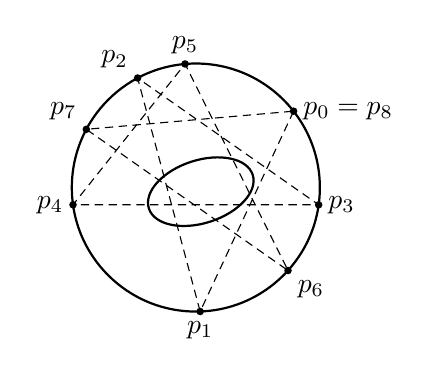
\begin{tikzpicture}[scale=1.05]
\draw[thick] (0,0) circle (1.5);
\begin{scope}[shift={(0.06,-0.05)},rotate=18]
\draw[thick] (0,0) ellipse (0.66 and 0.38);
\end{scope}
\coordinate (p0) at (38:1.5);
\coordinate (p1) at (-88:1.5);
\coordinate (p2) at (118:1.5);
\coordinate (p3) at (-8:1.5);
\coordinate (p4) at (188:1.5);
\coordinate (p5) at (95:1.5);
\coordinate (p6) at (-42:1.5);
\coordinate (p7) at (152:1.5);
\draw[densely dashed] (p0) -- (p1) -- (p2) -- (p3) -- (p4) -- (p5) -- (p6) -- (p7) -- cycle;
\foreach \pt in {p0,p1,p2,p3,p4,p5,p6,p7} \fill (\pt) circle (1.3pt);
\node[above] at (p5) {$p_5$};
\node[right] at (p0) {$p_0=p_8$};
\node[right] at (p3) {$p_3$};
\node[below right] at (p6) {$p_6$};
\node[below] at (p1) {$p_1$};
\node[left] at (p4) {$p_4$};
\node[above left] at (p7) {$p_7$};
\node[above left] at (p2) {$p_2$};
\end{tikzpicture}
\caption{\trPoncelet{}衍论（\mbox{19.10.8}）。（依原书手绘图重绘。）}\label{fig:poncelet-porism}
\end{figure}

\textbf{19.10.8.\ \trPoncelet{}衍论。}\ ——\ \emph{设 $C$ 与 $D$ 是 $\mathbb{R}^2$ 中的两个椭圆，$C$ 包含 $D$。在 $C$ 上任取一点 $p_0$。从 $p_0$ 向 $D$ 引的两条切线中任取一条，记作 $\ell_1$。于是 $\ell_1$ 总共与 $C$ 交于两点：$p_0$ 与另外一个点 $p_1$。从 $p_1$ 出发，向 $D$ 有两条切线，$\ell_1$ 与另一条直线 $\ell_2$。直线 $\ell_2$ 与 $C$ 交于另一个点 $p_2$。如此继续下去，便得到一个点列 $p_0$、$p_1$、$p_2$、$\dots$。设这个以 $p_0$ 为起点的序列是周期的，即对某个 $n$ 有 $p_0=p_n$。那么，以任意一点 $p\in C$ 为起点，它都是周期的（见图~\ref{fig:poncelet-porism}）。}

\trPoncelet{}衍论存在初等的证法，但一个牵涉椭圆曲线的证明相当漂亮，并且与一些更精致的思想建立起联系。我们不去证明\trPoncelet{}衍论，而是讨论几个相关的事实。

\textbf{19.10.K.（练习）}\quad 设 $E$ 是\trAlgClosedField{}上一条\trSmooth{}的\trDegree{} $3$ 射影平面\trCurve，$q$、$r\in E$，而 $n$ 是一个正整数。令 $F\colon E\to E$ 是\trMorphism{} $x\mapsto t(r,t(q,x))$。设对某个\trClosedPoint{} $p\in E$ 有 $F^n(p)=p$。证明：对一切点 $x\in E$ 都有 $F^n(x)=x$。

你应当感到一股想要改进这个结果的冲动。（你能证明：若对某个 $p\in E$ 有 $F^n(p)=p$，则 $F^n$ 是 $E$ 上的\trIdMorphism{}吗？你能把它推广到\trBaseField{}不\trAlgClosed{}的情形吗？）

\textbf{19.10.L.（练习）}\quad 设 $E$ 是 $\mathbb{R}^2$ 中的一个椭圆。对每个点 $(x,y)\in E$，存在另外一个点 $G(x,y):=(x,y')$（可能与原来那个点相同），它具有相同的第一个坐标，对应于过 $(x,y)$ 的竖直线与 $E$ 的「另一个」交点。类似地，存在另外一个点 $H(x,y):=(x',y)$，它具有相同的第二个坐标。令 $F=G\circ H$。证明：若对某个点 $p\in E$ 有 $F^{17}(p)=p$，则对一切点 $x\in E$ 都有 $F^{17}(x)=x$。（见图~\ref{fig:ellipse-staircase}，其中把 $17$ 换成了 $3$。）提示：这最好不用任何来自代数几何的花哨方法来做。

再说一次，你应当盼望改进这一点。这在多大的程度上依赖于实数？如果椭圆换成了另外一种圆锥截线呢？（这与\trEllipticCurve{}又有什么关系？这条圆锥截线为什么叫 $E$？！）

\begin{figure}[htbp]
\centering
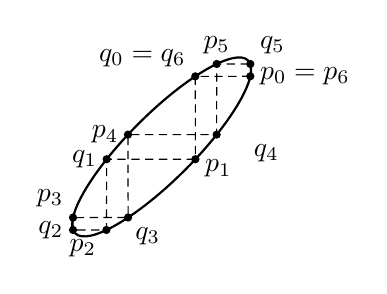
\begin{tikzpicture}[scale=1.15]
\begin{scope}[rotate=45]
\draw[thick] (0,0) ellipse (1.35 and 0.362);
\end{scope}
\coordinate (pa) at (0.979,0.780);
\coordinate (qa) at (0.371,0.779);
\coordinate (pb) at (0.372,-0.136);
\coordinate (qb) at (-0.607,-0.136);
\coordinate (pc) at (-0.610,-0.917);
\coordinate (qc) at (-0.979,-0.917);
\coordinate (pd) at (-0.979,-0.780);
\coordinate (qd) at (-0.371,-0.779);
\coordinate (pe) at (-0.372,0.136);
\coordinate (qe) at (0.607,0.136);
\coordinate (pf) at (0.608,0.916);
\coordinate (qg) at (0.979,0.916);
\draw[densely dashed] (pa) -- (qa) -- (pb) -- (qb) -- (pc) -- (qc) -- (pd) -- (qd) -- (pe) -- (qe) -- (pf) -- (qg) -- cycle;
\foreach \pt in {pa,qa,pb,qb,pc,qc,pd,qd,pe,qe,pf,qg} \fill (\pt) circle (1.3pt);
\node[right] at (pa) {$p_0=p_6$};
\node[above left] at (qa) {$q_0=q_6$};
\node[right, yshift=-0.12cm] at (pb) {$p_1$};
\node[left] at (qb) {$q_1$};
\node[below, xshift=-0.3cm] at (pc) {$p_2$};
\node[left] at (qc) {$q_2$};
\node[left, yshift=0.25cm] at (pd) {$p_3$};
\node[below, xshift=0.25cm] at (qd) {$q_3$};
\node[left] at (pe) {$p_4$};
\node[below right, xshift=0.35cm] at (qe) {$q_4$};
\node[above] at (pf) {$p_5$};
\node[above right] at (qg) {$q_5$};
\end{tikzpicture}
\caption{\mbox{练习~19.10.L}（把 $17$ 换成 $3$）。（依原书手绘图重绘。）}\label{fig:ellipse-staircase}
\end{figure}

\textbf{19.10.M.}\ \extrahard\ \textbf{（练习）}\quad 设 $k$ 是一个域，纯粹为了方便起见设它\trAlgClosed。设 $Q$ 是 $\mathbb{P}^3_k$ 中一个\trSmooth{}的\trQuadricSurface，而 $K$ 是 $\mathbb{P}^3$ 中的一个\trCone（一个\trRank{} $3$ 的二次曲面），使得 $E=Q\cap K$ 是一条\trSmooth{}\trCurve。
\begin{itemize}
\item[(a)] 证明 $E$ 的\trGenus{}为 $1$。
\item[(b)] 若 $\ell$ 是 $Q$ 上的一条直线，证明 $E$ 与 $\ell$ 交于两点（计重数）。
\item[(c)] 取定 $Q$ 的\trRuling{}（直线族）之一。证明：存在一个\trMorphism{} $G\colon E\to E$，它取 $E$ 的一个\trClosedPoint{} $p$，并把它送到含 $p$ 的那条\trRuling{}直线 $\ell$ 上 $E$ 的另外一个点。
\item[(d)] 利用 $Q$ 的另一族\trRuling，类似地定义 $H\colon E\to E$。取定一个正整数 $n$。令 $F=G\circ H$。证明：若对某一个\trClosedPoint{} $p\in E$ 有 $F^n(p)=p$，则对一切 $x\in E$ 都有 $F^n(x)=x$。
\end{itemize}

现在我们把\mbox{练习~19.10.M} 与\trPoncelet{}衍论（\mbox{19.10.8}）联系起来。令 $v$ 为 $K$ 的\trCone{}点。那么 $v\notin Q$，否则 $v$ 将是 $Q\cap K$ 的一个\trSingularPoint（你明白为什么吗？）。事实是：从 $v$ 出发的\trProjection{}给出一个\trMorphism{} $Q\to\mathbb{P}^2_k$，它在一条\trSmooth{}\trConic{} $D$ 之上分歧。（读完第 21 章之后，你或许能把这一点讲严格并加以证明。）$Q$ 上的诸直线投射为 $\mathbb{P}^2_k$ 中与 $D$ 相切的直线。从 $v$ 出发的\trProjection{}把 $K\setminus\{v\}$ 收缩成一条\trConic{} $C$。你或许能把\trPoncelet{}衍论（\mbox{19.10.8}）的论断（就这个 $C$ 与 $D$ 而言）用\mbox{练习~19.10.M} 的语言解读出来。（当心：\trPoncelet{}衍论（\mbox{19.10.8}）中的域不是代数闭的，而\mbox{练习~19.10.M} 中的域是代数闭的。）你甚至有可能取\trPoncelet{}衍论（\mbox{19.10.8}）中任意的 $C$ 与 $D$，按照\mbox{练习~19.10.M} 反向工程出 $K$ 与 $Q$，从而证明\trPoncelet{}衍论（并发现为什么在它的论断中藏着一条\trEllipticCurve）。
